\documentclass{standalone}
\usepackage{tikz-network}

\begin{document}
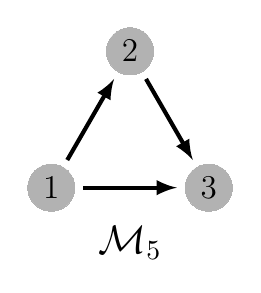
\begin{tikzpicture}

\SetVertexStyle[LineWidth=0, FillColor=black!30!white, LineColor=black!30!white, OuterSep=3, TextFont=\large]
\SetEdgeStyle[Color=black]
\SetTextStyle[TextFont=\Large]

\Vertex[x=4,label=1]{M_1}
\Vertex[x=5,y=1.732,label=2]{M_2}
\Vertex[x=6,label=3]{M_3}
\Edge[Direct](M_1)(M_2)
\Edge[Direct](M_2)(M_3)
\Edge[Direct](M_1)(M_3)
\Text[x=5,y=-0.7]{$\mathcal{M}_5$}

\end{tikzpicture}
\end{document}